Next, we measured file cache size. Our hypothesis is that file cache size is dynamic and it depends on amount of free memory available to the system. It wouldn't make sense for system to keep a lot of free pages around, when it could use them to speed up sequential reads.

To check our hypothesis we designed two controlled experiments with different amounts of free memory available to the system. One experiment runs with most of the memory unused. In another experiment, we allocate huge array and fill it with random data to avoid page sharing effects. We call this array \emph{balloon}. We used 10GB balloon in host environment and 3GB balloon in virtual machine.

Each experiment consists of four repeated sequential reads of varying size. We measure throughput on last three reads. If the read size is smaller than file cache size, the data accessed in repeated reads will be residing in cache, making repeated reads very fast. As soon as the size of our reads exceed cache size, we expect to see huge decrease in total throughput, since some of the repeated reads will need to go to disk and wait for I/O. Figure \ref{fig:p3pseudo} shows the pseudocode of experiments. We used 20MB buffer size, guided by insight from Section \ref{sec:p1}. In Virtual Machine environment we had to be careful to avoid effects of host file cache so we flushed it before every read.

\begin{figure}
\begin{algorithmic}
\STATE clear cache
\IF {ballooning enabled}
\STATE allocate huge array
\STATE fill the array with random data
\ENDIF
\STATE $size \leftarrow$ {sequential read size}
\STATE $file \leftarrow$ {huge file filled with random data}
\STATE $buffer\_size \leftarrow$ 20MB
\STATE flush the cache
\STATE read first $size$ bytes of $file$
\FOR{$i = 0$ to $3$}
\IF {running in VM}
\STATE clear host file cache
\ENDIF
\STATE open $file$
\WHILE{total bytes read $< size$}
\STATE start\_timer
\STATE read next $buffer\_size$ bytes
\STATE end\_timer and save the result
\ENDWHILE
\STATE close $file$
\ENDFOR
\STATE report average of all timers divided by $buffer\_size$
\end{algorithmic}
\caption{Function used to measure file cache size}
\label{fig:p3pseudo}
\end{figure}

Figure \ref{fig:p3graph} shows repeated read throughput for each measured sequential read size. We observe expected behavior for all four environments. First, we see sharp decrease in throughput after a certain point. We attribute this effect to read sizes getting bigger than the file cache. Next, we observe smaller file cache size when running experiments with ballooning, which proves our hypothesis that file cache size is dynamic and depends on free memory available to the system. The difference between the points of sharp decline in throughput for the cases with and without ballooning is exactly the size of the balloon. It is interesting to note that kernel didn't decide to swap out our balloon array and increase file cache size, even though that would speed up execution of our program. However, we can not make any inferences about general policy of swapping out memory to increase file cache size. (TODO maybe phrase this better)

\begin{figure}[ht!]
	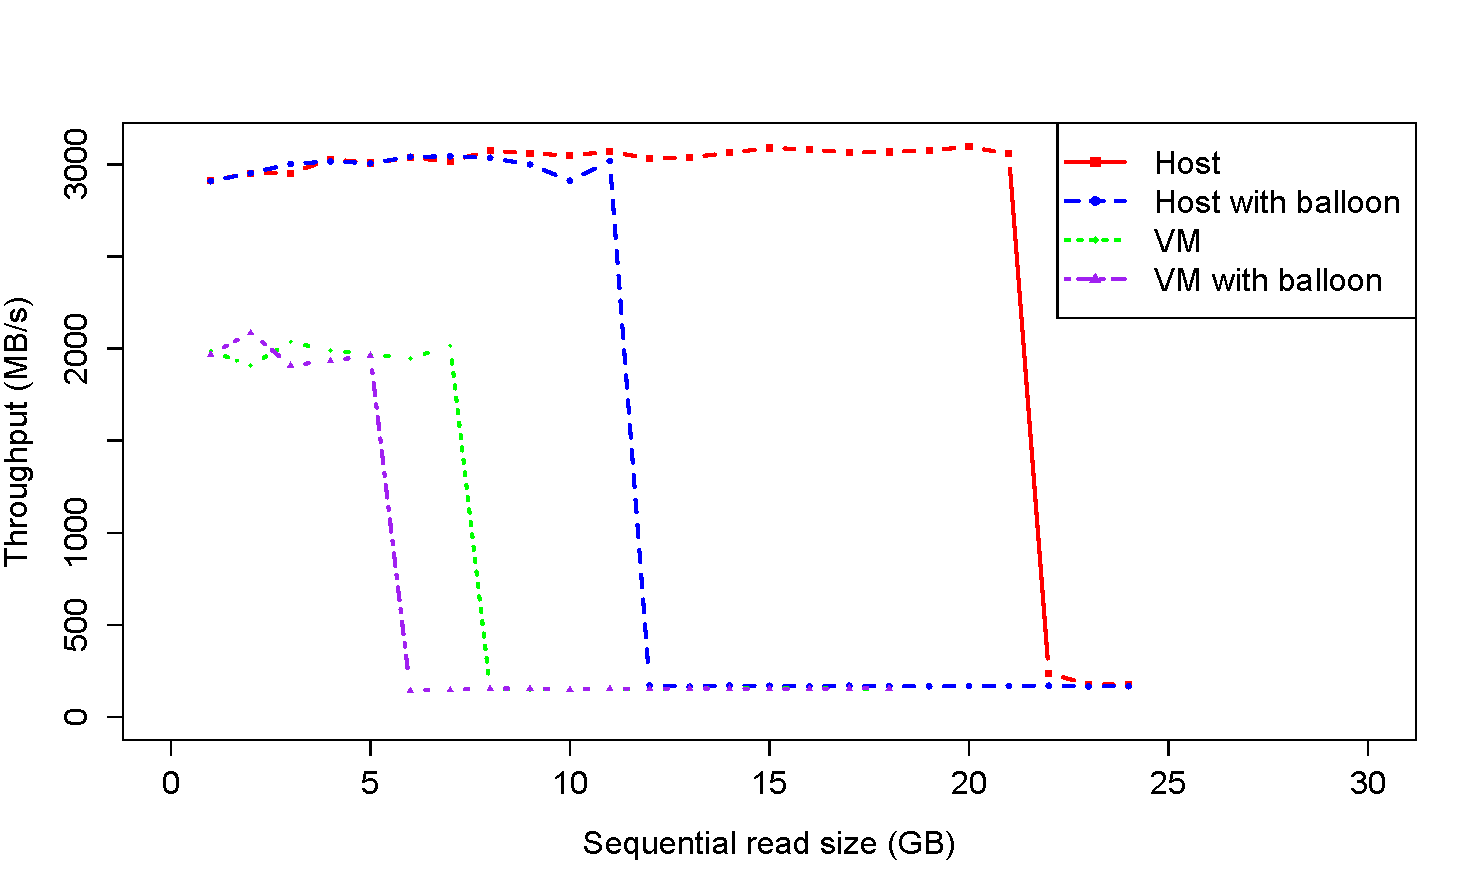
\includegraphics[width=0.5\textwidth]{./figures/p3.pdf}
	\caption{Repeated sequential read throughput. Horizontal axis shows size of repeated sequential read and vertical axis shows throughput. Throughput was measured in four environments: Host with a lot of free memory, Host with 10GB balloon, Virtual Machine with a lot of free memory and Virtual Machine with 3GB balloon.}
	\label{fig:p3graph}
\end{figure}
